\chapter[Metodologia]{Metodologia}

\section{Levantamento Bibliográfico}

Uma vez escolhida a área de interesse e o tema, a primeira etapa do trabalho consistiu em um levantamento bibliográfico, a fim de avaliar a disponibilidade de material para fomentar o tema de trabalho de pesquisa e também analisar o que já foi desenvolvido na área. Feito isso, tomando-se como base o que já foi publicado e desenvolvido, foram definidas as possíveis contribuições, identificando (como foi dito na Seção 1 \ref{introduc}) a limitação de desempenho e o desenvolvimento para \textit{mobile} como áreas a serem exploradas.  

\section{Equipamentos Utilizados}

O celular utilizado foi o \textit{Nexus} 4, o qual é o quarto  \textit{smartphone} da  \textit{Google}, projetado e fabricado pela \textit{LG Electronics}.  Ele possui o processador \textit{Snapdragon S4 Pro} de 1,512 GHz \textit{quad-core}, GPU ( \textit{Graphics processing unit}) \textit{Adreno} 320 e 2 GB de memória RAM. O computador utilizado foi o da linha \textit{Alienware} M14x fabricado pela \textit{Dell}, no qual possui processador \textit{Intel Core} i7 de 2,3 GHz, GPU \textit{NVIDIA GeForce} GTX de 2 GB e 8 GB de memória RAM. 

\section{Configuração do Ambiente}
\label{configamb}	

Em seguida, foram feitas as configurações dos ambientes de trabalho, em que  para desenvolver na plataforma \textit{Android} é necessário instalar o \textit{Android SDK} e o \textit{plugin} ADT, uma vez que seria utilizada a IDE \textit{Eclipse}. A biblioteca gráfica para sistemas embarcados \textit{OpenGL ES} já é oferecida pela plataforma \textit{Android}. Para computador, foi necessário instalar as bibliotecas \textit{GLUT}, \textit{GLEW} e por fim, a biblioteca gráfica \textit{OpenGL}. Para poder realizar a coleta de métricas, foram utilizadas as ferramentas (descritas nas subseções a seguir) \textit{Adreno Profiler}, pois o celular utilizado possui a GPU \textit{Adreno}, e a \textit{gDEBugger}, uma das únicas ferramentas gratuitas que suporta GPU's da empresa NVIDIA.

\subsection{\textit{Adreno Profiler}}

	A \textit{Adreno} é uma ferramenta que foca na otimização gráfica para celulares que possuem GPU Adreno (fabricada pela empresa \textit{Qualcomm}). De acordo com  \cite{adp}, a ferramenta provê suporte para \textit{Android} e \textit{Windows RT} (variação do sistema operacional \textit{Windows} 8  e projetada para \textit{devices} móveis), permitindo a otimização, análise por quadros e visualização de desempenho em tempo real. 

	Como pode ser visto na Figura \ref{adrenoProfiler}, a ferramenta possui um módulo de análise dos \textit{vertex} e \textit{fragment} \textit{shaders}, sendo possível editá-los e analisar os resultados de compilação em tempo real, além dela também gerar estatísticas.  

	\begin{figure}[h]
	\centering
		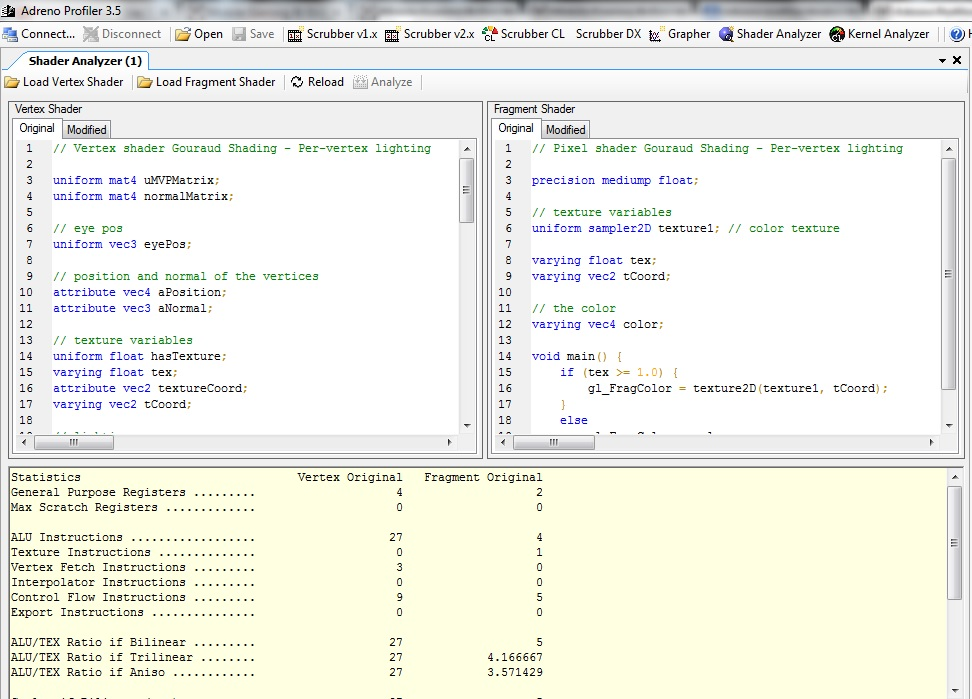
\includegraphics[keepaspectratio=true,scale=0.4]{figuras/shader_analyzer.jpg}
	\caption{Ferramenta \textit{Adreno Profiler}: analisador de \textit{shaders}}
	\label{adrenoProfiler}
	\end{figure}

	O módulo gráfico permite analisar algumas métricas, como a de quadros por segundo, onde na Figura \ref{graph} um gráfico é plotado em tempo de execução. Além disso, ela também exporta os resultados no formato CSV (\textit{Comma-Separated Values}), que consiste em um arquivo de texto que armazena valores tabelados separados por um delimitador (vírgula ou quebra de linha). O último módulo é o chamado \textit{Scrubber}, que provê informações detalhadas quanto ao rastreamento de uma chamada de função. 

	\begin{figure}[h]
	\centering
		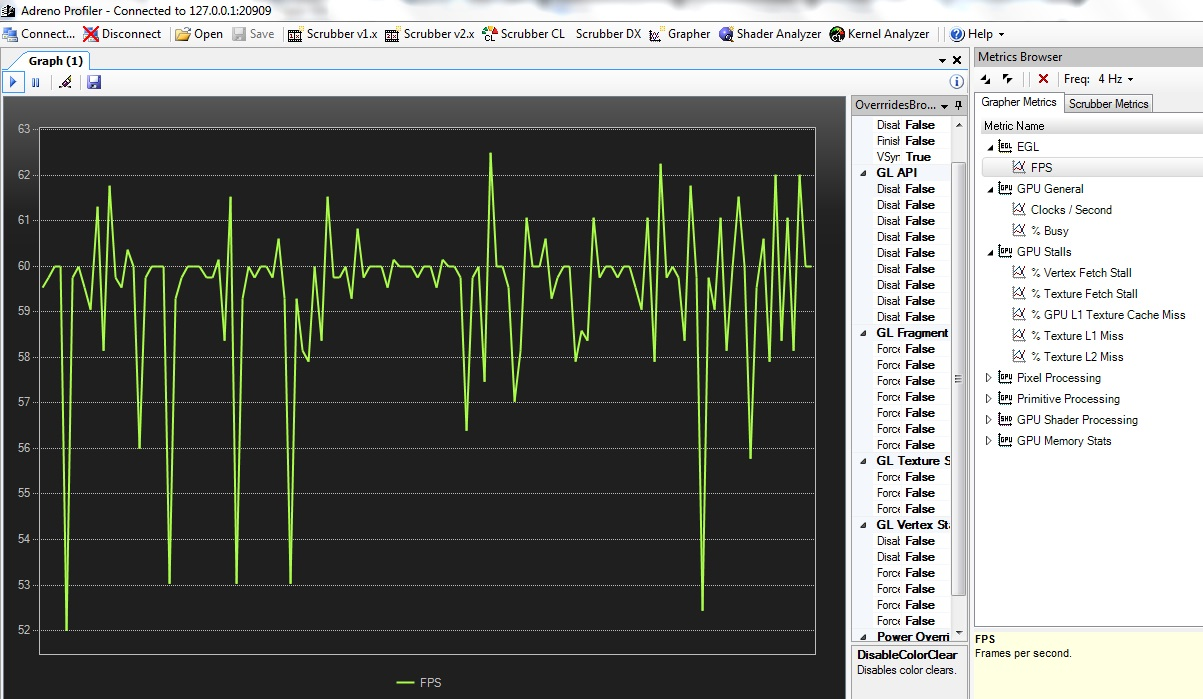
\includegraphics[keepaspectratio=true,scale=0.35]{figuras/graph.jpg}
	\caption{Ferramenta \textit{Adreno Profiler}: visualização de métrica quadros por segundo}
	\label{graph}
	\end{figure}


\subsection{\textit{gDEBugger}}
	
	A \textit{gDEBugger} é uma ferramenta de depuração e análise de desempenho (Figura \ref{gdebugger_fer}), que permite a rastreabilidade das chamadas \textit{OpenGL} de uma aplicação, disponível para \textit{Windows} e \textit{Linux}, com suporte às GPU's da empresa NVIDIA. Ela ajuda a encontrar  \textit{bugs}, melhorar o desempenho e consumo de memória de programas que utilizam a \textit{OpenGL}. 

	Como é mostrado em \cite{gdebugger}, é possível ver quais funções foram chamadas em um determinado quadro, o valor das variáveis da \textit{OpenGL} (como as matrizes de projeção, visualização e modelagem, por exemplo) e também mostrar medições com relação a quadros por segundo, consumo de memória, número de função de chamadas por quadro, entre outros. Além disso, ela (assim como a ferramenta \textit{Adreno Profiler}) também exporta os resultados no formato CSV.  

	\begin{figure}[h]
	\centering
		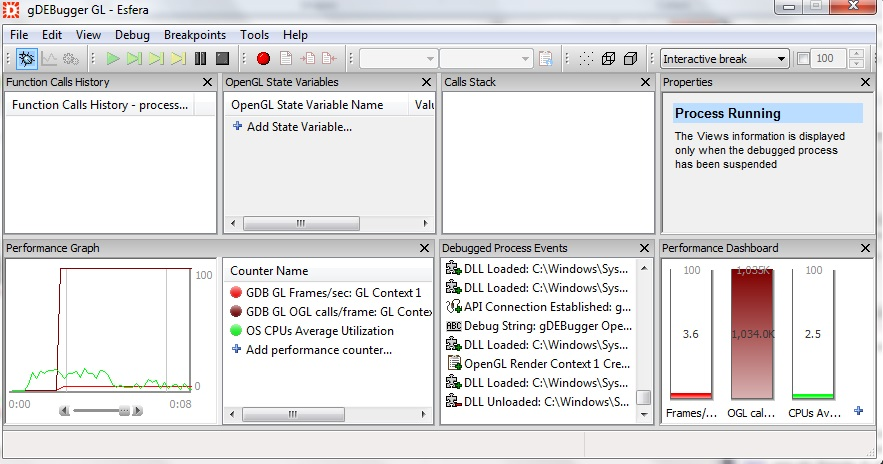
\includegraphics[keepaspectratio=true,scale=0.65]{figuras/gdebugger_fer.jpg}
	\caption{Ferramenta \textit{gDEBugger}: Gráfico de desempenho, histórico de chamadas, valor das variáveis e depuração}
	\label{gdebugger_fer}
	\end{figure}


\section{Ensaios Iniciais}

Primeiramente foi analisado se era factível estender o tema também para a plataforma \textit{Android} -- tanto no que diz respeito ao prazo quanto em relação ao conhecimento prévio da autora deste trabalho. Então avaliou-se o o nível de dificuldade de implementação de um  \textit{shader} para plataforma \textit{Android} (principalmente pelo fato da estudante não possuir experiência prévia com desenvolvimento \textit{mobile}), desenvolvendo um \textit{shader} simples aplicado num octaedro. Também desenvolveu-se o mesmo \textit{shader} para computador, analisando as as diferenças de implementação entre eles.  

Feito isto, também foi realizado um levantamento de ferramentas de otimização gráfica tanto para \textit{Android} como para computador, no qual escolheram-se as ferramentas \textit{Adreno} e \textit{gDEBugger}, respectivemente, as quais foram apresentadas na subseção Configuração do Ambiente. Essas ferramentas são utilizadas a fim de coletar medições quanto ao número de quadros por segundo de cada programa, utilizando um \textit{shader} específico, aplicado num objeto tridimensional com n número de polígonos. 

	Para testar a viabilidade do tema proposto, a ideia foi criar um programa constituído por objetos que fossem fáceis de variar o número de polígonos. Esses objetos escolhidos foram esferas pela facilidade de implementação, pois já existe uma função pronta da biblioteca \textit{glut} chamada \texttt{glutSolidSphere}, no qual se cria uma esfera baseada no tamanho do raio, número de cortes latitudinais e longitudinais. O número total de polígonos se dá pela multiplicação destes dois últimos parâmetros como é mostrado em \cite{poly}.  Além disso, estas esferas possuem diferentes movimentações, em que garante-se a ocorrência de oclusão entre elas e diferentes distâncias com relação à câmera. Feito isto, diferentes tipos de \textit{shaders} foram aplicados nestas esferas - a fim de posteriormente fazer medições com relação aos quadros por segundo - e finalmente poder traçar gráficos entre quadros por segundo \textit{versus} número de polígonos. Dessa forma foi possível analisar a complexidade algorítmica experimentalmente. Devido ao prazo, este experimento foi feito somente no computador, principalmente pela \textit{OpenGL ES} não possuir uma função equivalente à \textit{glutSolidSphere}, o que demandará mais tempo para implementá-la. 

	A seguir serão detalhados os \textit{shaders} escolhidos, implementados e analisados nos testes de viabilidade.

\subsection{\textit{Shader} cor vermelha}

	O \textit{shader} que define a cor para vermelha é muito simples,  seu \textit{vertex shader} apenas estabelece que a posição do vértice  se dá pelo pela multiplicação da coordenada (obtida utilizando o comando \texttt{gl\_Vertex} ) com a matriz de projeção, visualização e modelagem como é mostrada no Código \ref{codredvs}. 
	
	
	\lstinputlisting[language=C, caption = {\textit{Shader} cor vermelha:  \textit{vertex shader}}, label = {codredvs}]{codigos/red.vs}

	Já o seu \textit{fragment shader} (Código \ref{codredfs}) estabele que todo fragmento possui a cor vermelha, por meio da palavra restrita \textit{gl\_FragColor}.
	
	\lstinputlisting[language=C, caption = {\textit{Shader} cor vermelha:  \textit{fragment shader}}, label = {codredfs}]{codigos/red.fs}

	O resultado da aplicação deste \textit{shader} é mostrado na Figura \ref{red_shader}, em que a cor das esferas é vermelha e cada uma delas faz distintas movimentações. 

	\begin{figure}[h]
	\centering
		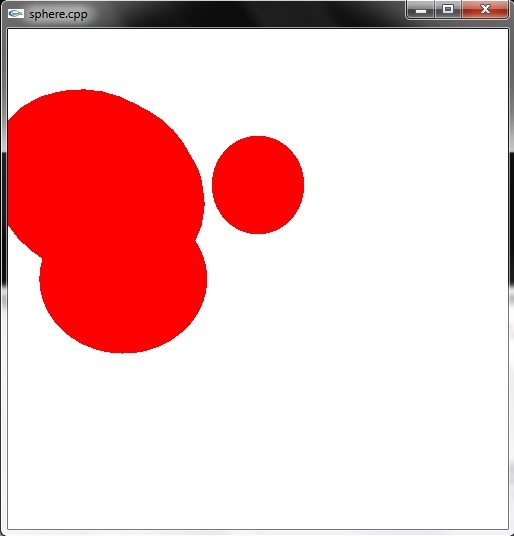
\includegraphics[keepaspectratio=true,scale=0.7]{figuras/red_shader.jpg}
	\caption{\textit{Red shader}}
	\label{red_shader}
	\end{figure}

\subsection{\textit{Flatten shading}}

	A ideia do \textit{flatten shading} é tornar o modelo tridimensional em bidimensional, achatado. Para isso,  a coordenada $z$ deve ser definida como zero. Mas para dar movimentação à malha do objeto, como mostrado no Código  \ref{codflatvs},  foi definida a variável  \textit{time} do tipo \textit{uniform} que é inicializada e passada pelo programa para o \textit{shader}. Assim, a coordenada z varia de acordo de acordo com o fator definido (que inclui esta variável).  

	\lstinputlisting[language=C,caption = {\textit{Flatten Shader}:  \textit{vertex shader}}, label = {codflatvs} ]{codigos/flat.vs}

	Neste caso o \textit{fragment shader} não interfere no resultado desejado, de modo que foi utilizado o mesmo do \textit{red shader}, definindo a cor para vermelha. A Figura \ref{flatten_shader} mostra as esferas achatadas, com a coordenada z variando de acordo com o fator definido. 

	\begin{figure}[h]
	\centering
		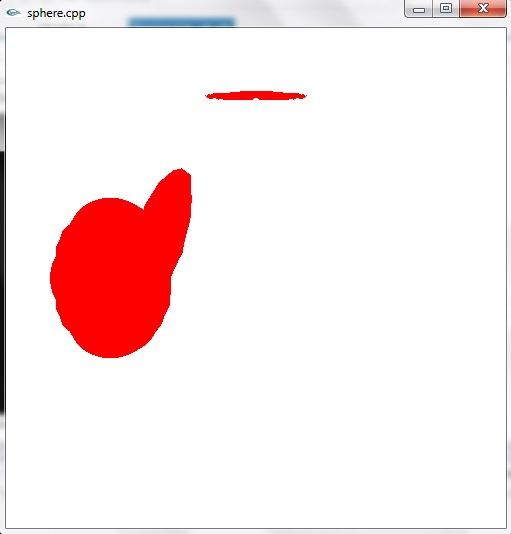
\includegraphics[keepaspectratio=true,scale=0.6]{figuras/flatten_shader.jpg}
	\caption{\textit{Flatten shader}}
	\label{flatten_shader}
	\end{figure}

\subsection{\textit{Toon shading}}

	O  \textit{toon shading} calcula a intensidade da luz por vértice para escolher uma das quatro cores pré-definidas. O Código  \ref{codtoonvs} é mostrado o cálculo da intensidade da luz por vértice, pegando primeiro a direção da luz (definida como uma variável \textit{uniform} passada pelo programa) para depois fazer o produto escalar entre ela e a normal (adquirida através do comando \textit{gl\_Normal}).  

	\lstinputlisting[language=C,label = {codtoonvs}, caption = {\textit{Toon Shader}:  \textit{vertex shader}} ]{codigos/toon.vs}

	A variável \textit{intensity} do tipo \textit{varying} é passada do \textit{vertex shader} para o \textit{fragment shader} para determinar qual das quatro cores será escolhida (Código \ref{codtoonfs}). 
  
 	\lstinputlisting[language=C, caption = {\textit{Toon Shader}:  \textit{fragment shader}}, label = {codtoonfs} ]{codigos/toon.fs}

	Assim, a direção da luz passada pelo programa é $(0 , 1 , 1)$ e o resultado da aplicação do \textit{shader} é mostrado na  Figura \ref{toon_shader}.

	\begin{figure}[h]
	\centering
		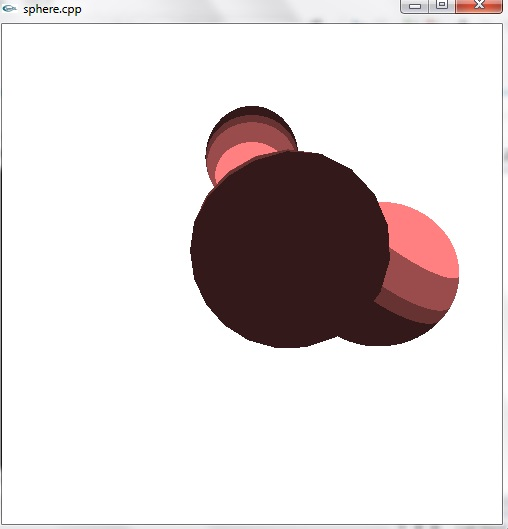
\includegraphics[keepaspectratio=true,scale=0.6]{figuras/toon_shader.jpg}
	\caption{\textit{Toon shader}}
	\label{toon_shader}
	\end{figure}

\subsection{\textit{Phong shading}}

	O \textit{vertex} e \textit{fragment shaders} do \textit{phong shading} implementam a técnica descrita na Seção \ref{flatgouphon}, em que primeiramente interpolam-se os valores das normais das primitivas e então computam-se os cálculos de luz para cada \textit{pixel}, utilizando as normais interpoladas. O Código \ref{codphongvs} e \ref{codphongfs} mostram as definições do \textit{vertex} e \textit{fragment shaders}, respectivamente, em que para isso é necessário definir as propriedades do material pelo programa.  

	\lstinputlisting[language=C, label = {codphongvs}, caption = {\textit{Phong Shader}:  \textit{vertex shader}}]{codigos/phong.vs}

	\lstinputlisting[language=C, caption =  {\textit{Phong Shader}:  \textit{fragment shader}}, label = {codphongfs}  ]{codigos/phong.fs}


	O resultado é mostrado na  Figura \ref{phong_shader}, o qual é muito parecido com o resultado padrão implementado pela  \textit{OpenGL}.

	\begin{figure}[h]
	\centering
		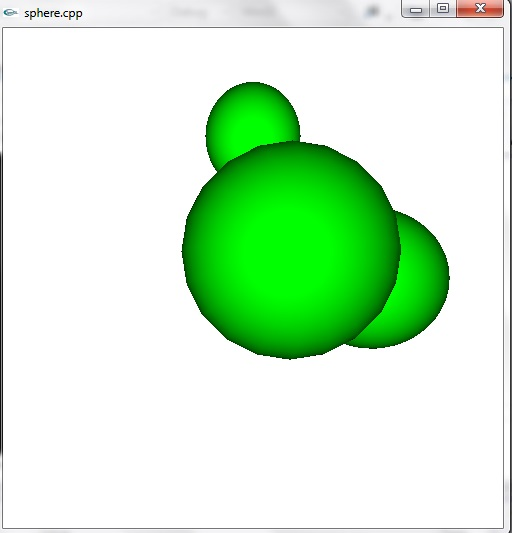
\includegraphics[keepaspectratio=true,scale=0.55]{figuras/phong_shader.jpg}
	\caption{\textit{Phong shader}}
	\label{phong_shader}
	\end{figure}

\subsection{\textit{Texture shading}}

	O \textit{vertex shader} do \textit{texture shading} primeiramente armazena as coordenadas de textura numa variável do tipo \textit{varying} (Código \ref{codtexvs}), e as repassa para o \textit{fragment shader}. Vale ressaltar que para este \textit{shader} foi necessário utilizar a função \texttt{gluSphere} ao invés da \texttt{glutSolidSphere}, pois ela permite especificar um objeto do tipo quádrico\footnote{Um objeto do tipo quádrico representa uma superfície quádrica, em que as coordenadas formam um polinômio de segundo grau de no máximo três variáveis, como por exemplo, as superfícies cônicas, esféricas e cilíndricas.}, que por sua vez dá opção de criar coordenadas de textura (utilizadas pelo \textit{shader}).  

	\lstinputlisting[language=C, caption =  {\textit{Texture Shader}:  \textit{vertex shader}}, label = {codtexvs} ]{codigos/tex.vs}

	No Código \ref{codtexfs}, o \textit{fragment shader} por sua vez, utiliza a textura passada pelo programa (Figura \ref{tex}) e aplica na coordenada repassada pelo  \textit{vertex shader}.

	\begin{figure}[h]
	\centering
		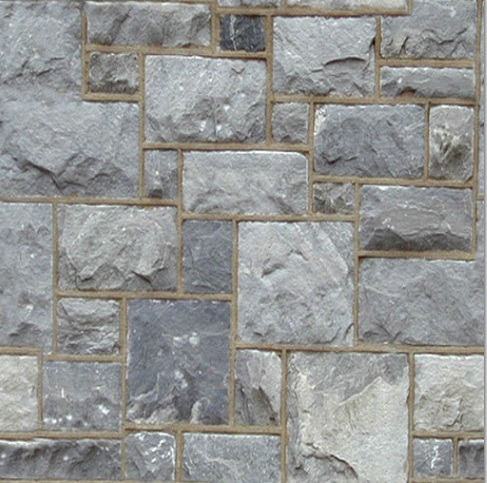
\includegraphics[keepaspectratio=true,scale=0.4]{figuras/tex.jpg}
	\caption{Textura utilizada}
	\label{tex}
	\end{figure}

	\lstinputlisting[language=C, caption = {\textit{Texture Shader}:  \textit{fragment shader}}, label = {codtexfs}]{codigos/tex.fs}

	O resultado é mostrado na  Figura \ref{texture_shader}.

	\begin{figure}[h]
	\centering
		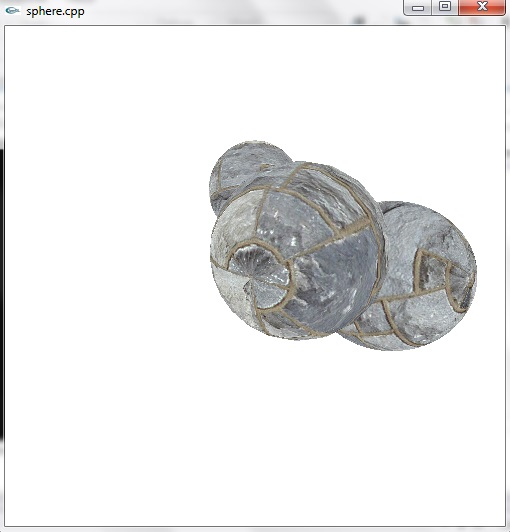
\includegraphics[keepaspectratio=true,scale=0.6]{figuras/texture.jpg}
	\caption{\textit{Texture shader}}
	\label{texture_shader}
	\end{figure}


 	Terminadas as implementações, foram utilizadas as ferramentas mencionadas anteriormente, sendoi possível coletar o número de quadros por segundo para diferentes números de polígonos. E dessa forma, gráficos (quadros por segundo \textit{versus} número de polígonos) para cada \textit{shader} implementado foram traçados, podendo então analisar experimentalmente suas complexidades algorítmicas.

\section{Implementação Plataforma \textit{Android}} 

	Para analisar a dificuldade de se implementar na plataforma \textit{Android}, codificou-se o \textit{Gouraud shader} descrito na Seção \ref{flatgouphon}, que utiliza a biblioteca \textit{OpenGL ES} e a linguagem de programação Java. Então o programa lê um arquivo  \textit{obj} (descrito na Seção \ref{formatobj}) e renderiza o modelo tridimensional utilizando a técnica de \textit{Vertex Buffer Object} descrita na Seção \ref{tecvertbuf} e o \textit{shader} mencionado. O resultado se encontra na  Figura \ref{android}.

	\begin{figure}[h]
	\centering
		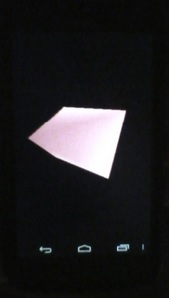
\includegraphics[keepaspectratio=true,scale=1.0]{figuras/android.jpg}
	\caption{Implementação plataforma \textit{Android}}
	\label{android}
	\end{figure}

	Este teste gerou a confiança de que seria possível implementar para a plataforma \textit{Android} dentro do prazo estipulado.  

\section{Implementação Computador}

	A fim de se ter uma comparação com o computador, já que a complexidade algorítmica não deve mudar no que diz respeito à ordem, codificou-se o mesmo programa mostrado na Figura \ref{computador} , porém utilizando a biblioteca OpenGL, Glut e a linguagem de programação C++.

	\begin{figure}[h]
	\centering
		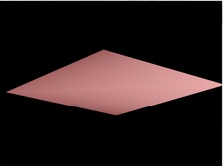
\includegraphics[keepaspectratio=true,scale=1.0]{figuras/computador.jpg}
	\caption{Implementação Computador}
	\label{computador}
	\end{figure}

\section{Procedimentos Futuros}

Assim, os próximos passos estão relacionados com a escolha de quais \textit{shaders} serão implementados e terão suas complexidades algorítmicas analisadas, como também com a modelagem de objetos tridimensionais possuindo diferentes números de polígonos e com a implementação do leitor do formato \textit{obj}. 

Por fim, o método dos mínimos quadrados será utilizado para poder estimar o número de quadros por segundo de um \textit{shader}, dado um número $n$ de polígonos, baseando-se na curva obtida experimentalmente pelos gráficos de cada \textit{shader} tanto no computador quanto no celular. 



